% !TeX document-id = {7d6761f7-6849-4b1b-9d26-a9263574efe4}
%!TeX TXS-program:compile = txs:///xelatex/
\documentclass{article}

\usepackage{fontspec}
%\setmainfont{D2Coding ligature}

\usepackage[hangul]{kotex}
\usepackage[hidelinks,unicode,bookmarks=true]{hyperref}
\usepackage{fancyvrb}
\usepackage{color}
\usepackage{graphicx}
\usepackage{amsmath}
\usepackage{amsthm}
\usepackage{amssymb}
%\usepackage{relsize}
\usepackage{centernot}
\usepackage[top=3cm, left=3cm, right=3cm, bottom=2cm]{geometry}
\usepackage{titling}
%\usepackage{lipsum}
\usepackage{standalone}
\usepackage{multirow}
\usepackage{wrapfig}
\usepackage{graphicx}
\usepackage{tikz}
\usetikzlibrary{quantikz}
\usepackage{braket}


\usepackage[linguistics]{forest}

\setlength{\droptitle}{-3em}

\newtheoremstyle{break}
{\topsep}{\topsep}%
{\itshape}{}%
{\bfseries}{}%
{\newline}{}%
\theoremstyle{break}
\newtheorem{defn}{Definition}
\newtheorem{thm}{Theorem}
\newtheorem*{coro}{Corollary}
\newtheorem{lemma}{Lemma}
\newtheorem*{remark}{Remark}
\newtheorem*{note}{Note}
\newtheorem*{prob}{Problem}
\newtheorem*{soln}{Solution}
\newtheorem*{claim}{Claim}
\renewcommand*{\proofname}{Proof}

\usepackage{hyperref}


\title{Quantum Speedup on S-DES Known Plaintext Attack\\\large 과목 75 최종보고서}

\author{2017320009 이상헌\\2017320023 조민규}

\date{\today}

\begin{document}
	\maketitle
	
	\section{서론}
	
	한 학기동안, Simplified DES에 대한 Known Plaintext Attack을 Quantum computer (simulator)을 사용하여 공격하는 방법에 관하여 연구하였다. 이를 위해 Microsoft Q\#을 사용하여 Quantum S-DES Oracle을 만들어 이에 Grover’s Algorithm을 적용시켰다.
	
	\section{연구 내용}
	
	Simplified DES는 Symmetric-key cryptosystem으로, DES와 유사한 구조로 되어 있지만, key size가 10bit, block size가 8 bit으로 줄어들고, 라운드 수 역시 2라운드로 줄어든 간략화된 구조로 되어 있다.
	
	S-DES의 경우 일반 컴퓨터를 사용해서도 공격을 하는 데에 오랜 시간이 걸리지 않는다. 하지만 S-DES는 그 전신인 DES와 유사한 구조로 되어 있고, classic logic gate(And, Or, Not, Xor 등)를 사용하기에 타 Symmetric-key cryptosystem에 이 방법을 적용시켜 활용할 수 있을 것으로 예상된다.
	
	타 cryptosystem을 사용하지 않고 S-DES을 선정한 이유는 비교적 작은 크기라는 점이 가장 크게 작용했다. 현재 상용화되어 있는 Quantum computer의 경우 사용 가능한 Qubit의 수가 굉장히 적고, 일반 컴퓨터에서 활용할 수 있는 Quantum simulator의 경우에는 Qubit의 수가 하나 증가할때마다 실행 시간이 두 배로 증가하여, 어느 쪽을 사용하든 상관없이 Qubit의 수가 적어야 실행이 가능하다는 문제점이 있다. 그렇기 때문에 DES, AES 등 Large-scale cryptosystem이 아닌 Small-scale인 S-DES를 선정하였다.
	
	\subsection{개별 연구 내용}
	공통적으로 학기 초반에 홍석희 교수님의 지도 하에 양자 컴퓨팅의 기초를 학습하였다.
    
	\subsubsection{조민규}
	
	Quantum S-DES Oracle에 대한 Theoretical Circuit Diagram을 만들었고, 이에 대한 Q\# implementation이 끝난 후 해당 circuit\footnote{Theoretical Circuit에서 Q\#에서 제공하는 feature으로 인해 몇몇 Gate가 삭제되거나 변형되었다.}에 대한 Gate analysis를 진행했다.
	
	\subsubsection{이상헌}
	
	Quantum S-DES Oracle과 그를 사용하여 key를 찾는 Grover's Algorithm을 Microsoft Q\#을 사용하여 구현했다.
	
	\section{연구 결과}
	
    \subsection{S-DES 양자 회로 구성}
	S-DES의 구조는 대부분이 permutation(또는 compression)이기 때문에 큰 문제가 되지 않는다. 하지만 Expansion과 S-Box의 두 부분에서는 문제가 될 수 있다. Expansion의 경우에는 CNOT gate를 사용하여 정보를 복사한다면 비교적 쉽게 해결할 수 있겠지만, S-Box의 경우에는 Lookup table으로 구성되어 있어 이에 대한 해결방안이 필요하다.
	
	그러기 위해 생각한 방안이 다음과 같은 회로를 사용한 Brute-forcing method이다:
	
	\begin{center}
		\begin{tikzpicture}
		\node[scale=0.6] {
			\begin{quantikz}
			\lstick{$\ket{In_3}$} & \gate{X} & \ctrl{1} & \qw & \qw & \qw & \qw & \qw & \qw & \ctrl{1} & \gate{X} & \qw  \rstick{$\ket{In_3}$} \\
			\lstick{$\ket{In_2}$} & \qw & \ctrl{3} & \qw & \qw & \qw & \qw & \qw & \qw & \ctrl{3} & \qw & \qw \rstick{$\ket{In_2}$} \\
			\lstick{$\ket{In_1}$} & \gate{X} & \qw & \ctrl{3} & \qw & \qw & \qw & \qw & \ctrl{3} & \qw & \gate{X} & \qw \rstick{$\ket{In_1}$} \\
			\lstick{$\ket{In_0}$} & \gate{X} & \qw & \qw & \ctrl{3} & \qw & \qw & \ctrl{3} & \qw & \qw & \gate{X} & \qw \rstick{$\ket{In_0}$} \\[0.2cm]
			\lstick{$\ket{0}$} & \qw & \targ{} & \ctrl{1} & \qw & \qw & \qw & \qw & \ctrl{1} & \targ{} & \qw & \qw \rstick{$\ket{0}$} \\
			\lstick{$\ket{0}$} & \qw & \qw & \targ{} & \ctrl{1} & \qw & \qw & \ctrl{1} & \targ{} & \qw & \qw & \qw \rstick{$\ket{0}$} \\
			\lstick{$\ket{0}$} & \qw & \qw & \qw & \targ{} & \ctrl{1} & \ctrl{2} & \targ{} & \qw & \qw & \qw & \qw \rstick{$\ket{0}$} \\[0.2cm]
			\lstick{$\ket{0}$} & \qw & \qw & \qw & \qw & \targ{} & \qw & \qw & \qw & \qw & \qw & \qw \rstick{$\ket{Out_1}$} \\
			\lstick{$\ket{0}$} & \qw & \qw & \qw & \qw & \qw & \targ{} & \qw & \qw & \qw & \qw & \qw \rstick{$\ket{Out_0}$}\\
			\end{quantikz}
		};
		\end{tikzpicture}
	\end{center}
	
	이 회로의 경우 S-Box 1에서 input으로 4(0010)가 들어왔을 때 output으로 3(11)이 나간다는 것을 표현하고 있다. 각 16개의 possibility에 대해 위와 같은 회로를 구성할 수 있고, 이를 연결하여 S-Box를 구현할 수 있다.
	
	다른 방법으로 Quine-McCluskey Algorithm을 통해 S-Box를 minimize 하여 And/Or/Not gate를 활용하는 방안을 생각할 수 있다. 하지만 이 경우 And/Or circuit은 모두 CCNOT gate를 활용해야 하고, 이를 활용하기 위해서는 Ancilla qubit, 즉 추가 Qubit이 필요하여 시공간적인 부담이 커지게 된다.
	
	이를 보완하기 위해 Quine-McCluskey Algorithm으로 minimize된 S-Box를 위의 Brute-forcing method와 비슷한 회로를 사용해 구현하는 Hybrid 방법을 생각해보았지만, 이를 직접 구현하지는 않았다. S-DES의 경우 Static S-Box를 사용하지만 Dynamic S-Box를 사용하는 Cryptosystem의 경우 Quine-McCluskey를 사용하는 것이 오히려 Time loss일 가능성이 생기기 때문이다.
	
	게이트 분석의 경우 실제 Quantum computer에서 Qubit 수의 제한이 없어진다면 가장 중요하게 사용될 Complexity의 Measure이기 때문에 그 개수를 각 게이트의 종류별로 세었다. Brute-force에서는 oracle call 1회당 40회의 CNOT gate, 188회의 Pauli-X gate, 66회의 CCNOT(Toffoli) gate를 사용하고, Hybrid에서는 40회의 CNOT gate, 172회의 Pauli-X gate, 26회의 CCNOT gate를 사용한다. Quine-McCluskey만을 사용하는 경우 Hybrid와 동일하거나 그보다 조금 많은 수준에서 그칠 것이나, Qubit 수에 제한이 있는 현재로서는 사용할 수 없는 방법이기 때문에 계산하지 않았다.
	
    \subsection{Microsoft Q\# 기반 S-DES 구현체}
    초기에는 다음과 같이 34개의 qubit을 사용하여 구현하였다.
    \begin{itemize}
        \item 입력 키에 10-qubit
        \item 암호화 오라클 용도 1-qubit
        \item 암호화 중간과정의 8-qubit
        \item expanded plaintext(EP)를 위한 8-qubit
        \item S-Box 결과 저장 용도 4-qubit
        \item S-Box에서 사용할 여분의 3-qubit
    \end{itemize}
    
    \begin{wrapfigure}{r}{0.4\textwidth}
        \centering
        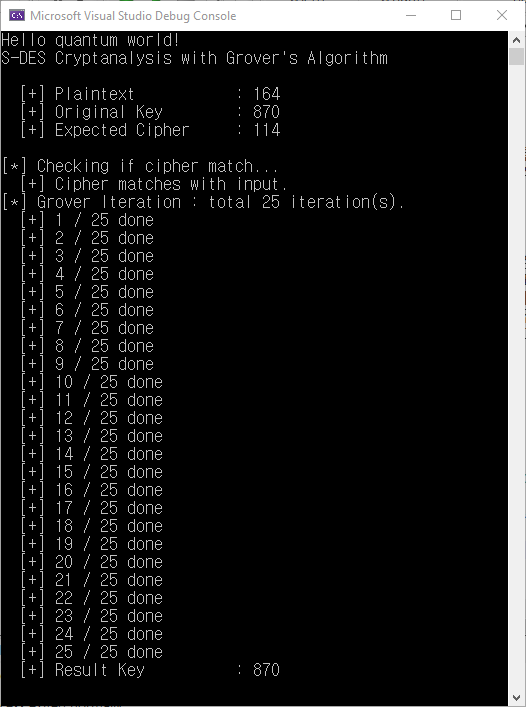
\includegraphics[width=0.4\textwidth]{./qsharp_exec.PNG}
        \caption{구현체 실행 화면}
        \label{fig:qsharp_exec}
    \end{wrapfigure}
    
    프로그램이 48GB를 할당하고 비정상 종료되어 최대한 큐빗의 개수를 줄이는 방향을 택했고, 네 가지 요인으로 줄일 수 있었다. 첫째로 암호화 중간과정의 qubit은 input plaintext qubit을 그대로 이용하면 되기에 필요하지 않았다. 둘째로 expanded plaintext 때문에 qubit을 복제할 필요 없이, 각 S-Box별로 따로 계산할 수 있다는 성질을 이용하였다. 셋째로 S-Box를 독립적으로 계산하면서 필요한 qubit의 개수가 4개에서 2개로 감소하였다. 넷째로 위에서 나왔던 brute-forcing method에서 필요했던 3개의 ancilla qubit을 Microsoft Q\#의 controlled functor를 이용해 제거하였다.
    
    결과적으로 프로그램에 필요한 qubit은 21개이다.
    \begin{itemize}
        \item 입력 키에 10-qubit
        \item 암호화 중간과정의 8-qubit
        \item 암호화 오라클 용도 1-qubit
        \item S-Box 결과 저장 용도 2-qubit
    \end{itemize}
    구현 결과 Grover's Algorithm까지 포함하여 암호화 오라클을 26번 호출하는 과정이 약 72초 소모되어, 한 오라클 쿼리에 약 2-3초 내외 소모되었다. 메모리도 최대 54 MB 정도를 차지하였다. 실행 화면은 그림 \ref{fig:qsharp_exec}과 같다.
    
	\section{향후 연구 계획}
	
	해당 implementation에 대해서 가장 문제가 되었던 부분은 임의의 Plaintext $P$, Ciphertext $C$쌍에 대해 $\{K|C=SDES(P,K)\}$ 의 크기, 즉 Key count가 다르다는 것에 있었다. 그러나 선행 연구에서 해의 개수가 알려지지 않았을 때도 효율적으로 Grover iteration을 수행하면 최적의 시간 복잡도로 계산할 수 있음이 알려져 있었다. 때문에 추후 연구 과제는 홍석희 교수님과의 면담을 통해 이어서 진행해볼 예정이다.
	
    \section*{별첨}
    
    별첨 문서의 목록은 다음과 같다.
    \begin{itemize}
    \item \verb|./cisc| : 2020 한국정보보호학회 한국정보보호학회 하계학술대회(\url{http://www.cisc.or.kr/})에 제출한 최종논문이 포함되어 있다. 본 연구의 핵심과 참고 문헌이 기술되어 있다.
    \item \verb|./qsharp| : Microsoft Q\#으로 작성한 S-DES 암호화 알고리즘 및 Grover's Algorithm 프로젝트 파일이 포함되어 있다. Grover's Algorithm 코드는 \url{https://github.com/microsoft/QuantumKatas/blob/master/GroversAlgorithm/ReferenceImplementation.qs}을 참고하였다.
    \item \verb|./presentation.pdf| : 연구를 진행하면서 작성해온 발표 자료이다.
    \item \verb|./py_sdes| : Python으로 구현한 S-DES이다. \verb|sdes.py|를 통해 암호화를 할 수 있고 \verb|attk.py|를 통해 brute-force를 통해 평문과 암호문이 주어졌을 때 해당하는 key를 전부 구할 수 있다.
    \end{itemize}
\end{document}